\documentclass[12pt]{scrartcl}

\include{amsfonts,amssymb,amsmath,amsthm,txfonts,pxfonts,mathrsfs,enumitem}
\usepackage[headheight=15pt,paperwidth=8.5in, paperheight=11in,margin=0.75in]{geometry}
\usepackage{lastpage}
\usepackage{fancyhdr}

\usepackage{mathtools}
\DeclarePairedDelimiter\floor{\lfloor}{\rfloor}
\newcommand{\argmax}{\mathop{\mathrm{argmax}}} 
\newcommand{\argmin}{\mathop{\mathrm{argmin}}} 

\newcounter{teamnumb}
\setcounter{teamnumb}{54301}

\ttfamily{
\lhead{Team\ \# \theteamnumb}\rhead{Page \thepage\ of \pageref{LastPage}}}
\cfoot{}
\renewcommand{\headrulewidth}{0pt}
\pagestyle{fancy}

\title{\vspace{-1.7cm} Emerging Markets: Comparing University Poverty Alleviation with Charitable Education Donations}
\subtitle{A Model for Post-Secondary Investments\vspace{-1.3cm}}

\begin{document}
\maketitle
\thispagestyle{fancy}

\section*{Summary}



\newpage
\tableofcontents
\newpage
	

\section{Introduction}
	\subsection{The Problem}
		The Goodgrant Foundation is a charitable organization with a mission to improve educational performance of students attending colleges and universities in the United States. The foundation intends to donate a total of 100,000,000 USD to a group of schools each year, for five years. They also wish to avoid investing in universities that have already received grants from major charitable organizations such as the Gates and Lumina Foundation.\\
		
		We present a mathematical model to outline an ranking and investment strategy to provide the maximal return on investment(ROI) appropriate for an education charity.  The model is split into two sections and is applicable in choosing $1\cdots N$ institutions. \\

The first section outlines determining bench mark points and comparing the rest of the institutions to them via a k-Nearest Neighbours(k-NN) Algorithm. In the second section, we derive a ROI measuring the effect the grant would have on improving student performance. In particular, our ROI reflects changes in terms of incoming poverty and outgoing poverty. In the Model Testing section, we input a subset of the U.S. National Center on Education Statistics data set and College Scorecard data set and output a list of $1,\cdots{N}$ schools, the investment amount, and number of students affected. In Sensitivity Analysis, we restrict the distance in the kNN algorithm to obtain a subset of our prioritized schools and assess the model's stability. Lastly, we summarize the findings of the paper and suggest future additions. 
	
	\subsection{Assumptions and Rationale/Justification}
	\begin{itemize}
		\item \textbf{The Gates Foundation and Lumina Foundation will continue to donate to the same school for at least two years:} Typically large charities often donate sums over the course of number years to allow highest impact. \cite{Conkey} We are able to remove those particular schools from our candidate list to avoid duplicating the two foundation efforts. 
				
		\item \textbf{Students who receive a grant will stay in the program and successfully graduate:} There are many factors that could cause students to not be able to graduate, but we will focus on financial support because it is the root of other factors..\cite{Trom}

		\item \textbf{} 
	\end{itemize}
	
	\subsection{Summary of our Approach}
		\begin{itemize}
		\item Create a benchmark setting: top 20 schools that we consider to have good performance. Each school represent a class.  
		\item Identify universities that have similar characteristics to the benchmark list. 
		\item Prioritize universities to be invested in by the amount of grants they received from other sources.
		\item Determine the amount of investment and allocation to maximize the return on investment. 
		\end{itemize}
				 
\clearpage
\section{Model Design and Approach}
	\subsection{Notations and Definitions}
	\begin{enumerate}
		\item $U_j^{[i]} = $ university $j$ of class $i$
		\item $U_o^{[i]} = $ benchmark university for class $i$
		\item $A_j^{[i]} = $ amount invested in university $j$ for class $i$
		\item $T_j^{[i]} = $ Tuition in university $j$ for class $i$
		\item $n_j^{[i]} = $ number of students receving our grant in university $j$ for class $i$
		\item $IP_j^{[i]} = $ poverty rate of students entering university $j$ for class $i$
		\item $OP_j^{[i]} = $ poverty rate of students exiting university $j$ for class $i$
		\item $\phi_j^{[i]} = $ number of students in university $j$ for class $i$
		\item $\Phi = $ Total number of universities
		\item $g_j^{[i]} = $ maximum amout of grants to be given to university $j$ for class $i$
		\item \underline{Group}, refers to the Carnegie Classification of the university
		\item \underline{Class}, refers to which benchmark within the group, the university is closest to.
	\end{enumerate}
	
	\subsection{Benchmark Selection}
	
	First we omitted any below medium size universities or communal universities such as racial or religious schools. Then we partition all universities by number of years required for graduation. Lastly, we rank the universities by the amount of their poverty elevation standards: \\ \\ 
	$$
		R_j^{[i]}=\frac{IP_j^{[i]}-OP_j^{[i]}}{IP_j^{[i]}}
	$$  
	Next we choose the top, highest ranking universities per `years of graduation'-group. We set these chosen universities as our benchmarks for each class in each group.\\
	
	i.e.
	$$
		o^{[i]} = \argmax_{j} R_j^{[i]}
	$$
	Where $o$, is to represent the benchmark index of the class $i$.

	\subsection{Categorizing Institutions into Classes}
	
	We aim to classify each university into some class $i$. This is done via the kNN algorithm: a non-parametric method used in classification supervised learning problems. The output is determined by a majority vote, where the object is assigned to the class most common with it's neighbours. \cite{Hastie}\\

We set up the following model:
Assuming $j\in [1,n]$,where $n$ = amount of variables. For a detailed selection list please see Appendix 1. Let $y_j^{[i]}$ be the $j$-th variable for the $i$-th class benchmark. Let $x_j$ be the $j$-th variable of a particular university. A university $u$, is considered a member of the $k$-th class if the variables $x_i$ of that university is `close' to a particular variable of a given class in euclidean-space.\\
	
That is, if $u$ belongs to the $k$-th class then
	$$
		k = \argmin_{i} \sqrt{ \sum_{j=1}^n (x_j-y_j^{[i]})^2 }
	$$

	
	\subsection{Investment Strategy}

	\subsubsection{Number of student-Helped}
		Let $A_j^{[i]}$ be the amount we invest in university $j$ of the class $i$, and $T_j^{[i]}$ be the tuition of low-income students. Then we can compute the number of students who we help as:

		\begin{align*}
			n_j^{[i]} &= \floor{\frac{A_j^{[i]}}{T_j^{[i]}}}\\
			n^{[i]} &= \sum_{j=1}^\infty n_j^{[i]}\\
			n &= \sum_{i=1}^\infty n^{[i]}
		\end{align*}
		Please note that the number of universities is \underline{finite}, we use infinity here in order to avoid the introduction of more variables.\\

	\subsubsection{Adjusted Poverty}
		Next we computed the adjusted poverty rate. We make a crucial assumption here about the correlation between grant-money and retention rates. We assume that every student who receive the grant will stay in the program and university (this assumption can be adjusted by a future study on the subject matter).\\
		\\
		Let $\phi_j^{[i]}$ be the total number of students in university $j$ for class $i$.\\
		The adjusted rate of existing poor students based on our assumptions is:
		\begin{equation}
			OP_j^{[i]*} = \frac{  OP_j^{[i]}\phi_j^{[i]}-n_j^{[i]}  }{ \phi_j^{[i]}  }
		\end{equation}
		
		We can then provide a rank to this university, in the similar fashion we computed the rank for the benchmark universities:
		$$
			R_j^{[i]*}=\frac{IP_j^{[i]}-OP_j^{[i]*}}{IP_j^{[i]}}
		$$
		We use this to compute the increase to the social well-being of students going to this university. 

	\subsubsection{Return on Investment (ROI)}
		The return on investment for our model will be the change in the level of alleviation of poverty provided by our investment.\\
		We do this as follows:
		\begin{equation}
			R_j^{[i]}(1+r_j^{[i]}) = R_j^{[i]*}
		\end{equation}
			
		where $r_j^{[i]}$ is the return on investment for a particular school.\\
		We also note that (2) can be rewritten as:
		
		\begin{equation}
		r_j^{[i]} = \frac{ OP_j^{[i]} - OP_j^{[i]*}  }{ IP_j^{[i]} - OP_j^{[i]}  }
		\end{equation}	
	 	This will later be used for simplification purpose of the maximization problem.\\
		\\
		We then average these rates, to get the approximated return:
		$$
			\bar{r} = \frac{ \sum_{j=1}^\infty\sum_{i=1}^\infty r_j^{[i]}  }{ \# (\{ \forall i, j :  U_j^{[i]} \}) }
		$$
		For simplification, the total number universities, or $\# (\{ \forall i, j :  U_j^{[i]} \})$ will be written as $\Phi$, so
		$$
			\bar{r} = \frac{ \sum_{j=1}^\infty\sum_{i=1}^\infty r_j^{[i]}  }{ \Phi }
		$$

	\subsubsection{Maximization of return}
		Now that we have a measure of return on investment, we wish to maximize this measure based on the physical restriction that are given to us.\\
		Since we only have a limit of \$$100$M, and would not want to overshoot our investment by giving any particular university more than what the top-tier schools are given. We put the following restriction forth.\\
		\\
		Let $g_j^{[i]} = \max( \frac{  G_o^{[i]}  }{  \phi_o^{[i]} } - \frac{  G_j^{[i]}  }{  \phi_j^{[i]} } \ ,\ 0 )$, be the restriction on the per-student investment.\\ 
		We do this, in order to make sure that our investment has a reasonable bound that does not exceed the higher-tiered school.\\
		\\
		So now our problem can be formulated as follows:
		\begin{equation*}
				\begin{aligned}
					& \underset{A}{\text{maximize}}
					& &\bar{r}\\
					& \text{subject to}
					& & \sum \sum A_j^{[i]} = 100,000,000 \\
					&&& \forall i,j \ \ \ 0\le A_j^{[i]} \le g_j^{[i]}\phi_j^{[i]}
				\end{aligned}
		\end{equation*}

	\subsubsection{Simplifying the complexity}
		In order to simplify the complexity of the previous problem we outlined before. We reformulated the problem as follows:\\
		First, recall (1) and (3) which can be further simplified into:
		
		\begin{equation}
			\begin{aligned}
			r_j^{[i]} &= \frac{1 }{ \phi_j^{[i]} (IP_j^{[i]} - OP_j^{[i]} ) } n_j^{[i]} = \Delta_j^{[i]} n_j^{[i]}
			\end{aligned}
		\end{equation}	
		We note that $\Delta_j^{[i]}$ from (4) is the information given by our data. It must be positive as $$\Delta_j^{[i]}\implies IP_j^{[i]} < OP_j^{[i]}$$
		Which means that the considered university is getting more in funding than the benchmark one. If this happens, we omit that university from our dataset.\\ 
		\\
		Whereas $n_j^{[i]}$ is the number of students we invest in, which is a variable that will be controlled by us.\\
		\\
		Hence the mean return can be written as:
		\begin{align*}
			\bar{r} &= \sum_{j=1}^\infty\sum_{i=1}^\infty \frac{ 1  }{ \Phi } r_j^{[i]} = \frac{ 1  }{ \Phi }\sum_{j=1}^\infty\sum_{i=1}^\infty \Delta_j^{[i]}n_j^{[i]}
		\end{align*}
		So our new maximization problem can be formulated as follows:
		\begin{equation*}
				\begin{aligned}
					& \underset{\forall n_j^{[i]}}{\text{maximize}}
					& &\frac{ 1  }{ \Phi }\sum_{j=1}^\infty\sum_{i=1}^\infty \Delta_j^{[i]}n_j^{[i]}\\
					& \text{subject to}
					& & \sum \sum n_j^{[i]}T_j^{[i]} = 100,000,000\\
					&&& \forall i,j \ \ \ 0\le n_j^{[i]} \le \frac{g_j^{[i]}\phi_j^{[i]}}{T_j^{[i]}}
				\end{aligned}	
		\end{equation*}
		
\section{Model Application} 
	As discussed in the previous section, the first goal in the analysis is to find a list of benchmark schools. However, before doing so, we partitioned the schools by the type of degrees that they predominantly provide. This was due to the fact that otherwise, many pieces of data become `null', and the kNN algorithm becomes biased towards schools that have less-years-to-graduation.\\ 
	\\
	Once the partitioning was done, we applied the poverty alleviation rank (PAK). Which was inspired by the results of Trombitas \cite{Trom} and College-Score Card \cite{US}.\\
	\begin{figure}[h]
		\centering
		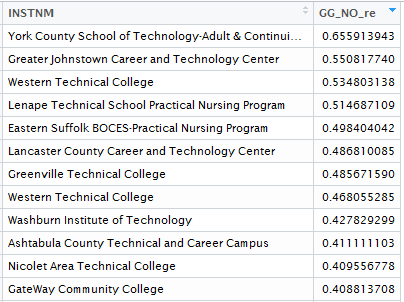
\includegraphics[width=0.5\textwidth]{2yr-col.png}
		\caption{2 year program}
		\label{fig:prog2}
	\end{figure}
	\begin{figure}[h]
		\centering
		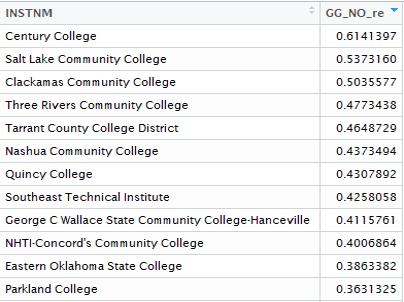
\includegraphics[width=0.5\textwidth]{4yr-col.png}
		\caption{Bachelor program}
		\label{fig:prog4}
	\end{figure}
	\begin{figure}[h]
		\centering
		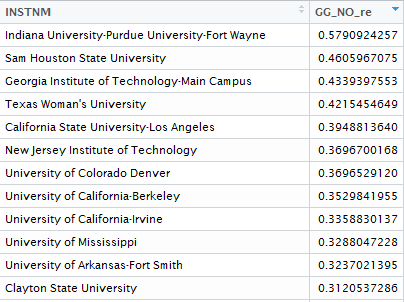
\includegraphics[width=0.5\textwidth]{6yr-col.png}
		\caption{Grad program}
		\label{fig:prog2}
	\end{figure}
	Once we acquired this data, we chose the top 10 schools from each school type as our benchmark schools. Since we did not want to overlap with grants given by other institutions, we filtered the next list using the data given by the Gates\cite{Bill} and Lumina \cite{Grant} Foundations.\\
	\\
	As this point, we used the kNN algorithm as the method of selection for the nearest best schools. As we wish to avoid investing in the top tier schools, and would rather invest in schools with the potential to become the top-tier.\\ 
	Prior to the application of the kNN algorithm we had to normalize the data by transforming each variable to a scale in $[0,1]$, as otherwise variables measure in larger values would be favored to smaller variables.\\
	\\
	This identification provided us with the following schools (please note that this is not the entire dataset, the full dataset will be provided separately) \ref{fig:kNN}.
	\begin{figure}[h]
		\centering
		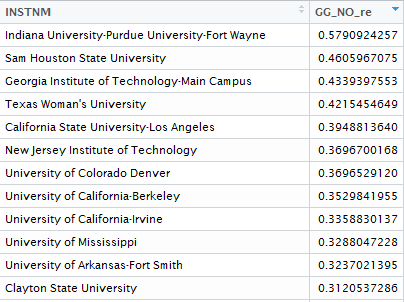
\includegraphics[width=0.6\textwidth]{6yr-col.png}
		\caption{Sample of kNN results}
		\label{fig:kNN}
	\end{figure}

\section{Discussion} 
\subsection{Sensitivity Analysis}
In order to test model stability, we impose a radius condition to the kNN selection algorithm. The model testing outlined in Section 3 used an unrestricted subset of the data. We compute the the mean and standard deviation for each class $i$. Then each value exceeding k from k = 1,..3 standard deviations away was omitted from the data passed to the investment algorithm. The goal is to partition the dataset such that the subset data will have 68\%, 95\%, and 99.7\% of the data.\\

With all other variables the same the ROI for each standard deviation(STD) is:
\begin{enumerate}
\item STD 1 ROI: 0.0353
\item STD 2 ROI: 0.0499
\item STD 3 ROI: 0.0474
\end{enumerate}

All ROI are relatively the same suggesting that the model does well with any size of data input. 

\subsection{Strengths}
\subsection{Weaknesses}

\section{Conclusions}
\clearpage

\section{Letter to Mr. Alpha Chiang}
Dear Mr. Alpha Chiang,


\newpage



\begin{thebibliography}{10}
	\bibitem{Trom} Trombitas, Kate.  \emph{Financial Stress: An Everyday Reality for College Students}. Inceptia, July 2012. PDF. 

	\bibitem{Carnevale} Carnevale, Anthony, Ban Cheah, and Martin Van Der Werf. \emph{Ranking Your College}. Georgetown University Center on Education and the Workforce, Dec. 2015. PDF.
	
	\bibitem{Conkey} Conkey,Christopher 2006. ``Big donations to charity often include spending advice” \emph{The Wall Street Journal Asia} 05:
	
	\bibitem{Bill} ``Bill \& Melinda Gates Foundation." \emph{Bill \& Melinda Gates Foundation}. Web. 29 Jan. 2016. 
	
	\bibitem{Grant} ``Grants Database." \emph{Grants Database}. Web. 29 Jan. 2016. $<$https://www.luminafoundation.org/grants-database/strategy/student-financial-supports$>$. 
	
	\bibitem{Hastie} Hastie, Trevor, Robert Tibshirani, and Jerome Friedman. ``Prototype Methods and Nearest-Neighbors". \emph{The Elements of Statistical Learning: Data Mining, Inference, and Prediction.} 2nd ed. New York: Springer, 2009. Print. 

	\bibitem{IPEDS} ``IPEDS Data Center." \emph{IPEDS Data Center.} Web. 30 Jan. 2016. \textless https://nces.ed.gov/ipeds/datacenter/DataFiles.aspx\textgreater.

	\bibitem{Wayne} Hanushek, Eric and Margaret Raymond. 2005. ``Does School Accountability Lead to Improved School Performance?” \emph{Journal of Policy Analysis and Management} 24(2): 297-329.
	
	\bibitem{Winston} Winston, Wayne L. ``Linear Programming."  \emph{Operations Research: Applications and Algorithms}. 4th ed. Belmont, Calif.: Duxbury, 2003. Print.
	
	\bibitem{US} ``Using Federal Data To Measure And Improve The Performance Of U.S. Institutions of Higher Education" Sept 2015. \textless https://collegescorecard.ed.gov/assets/UsingFederalDataToMeasureAnd- \\ImprovePerformance.pdf\textgreater.
\end{thebibliography}
\end{document}
